\documentclass[a4paper]{article}

%% Language and font encodings
\usepackage[english]{babel}
\usepackage[utf8x]{inputenc}
\usepackage[T1]{fontenc}

%% Sets page size and margins
\usepackage[a4paper,top=3cm,bottom=2cm,left=3cm,right=3cm,marginparwidth=1.75cm]{geometry}

%% Useful packages
\usepackage{amsmath}
\usepackage{graphicx}
\usepackage[colorinlistoftodos]{todonotes}
\usepackage[colorlinks=true, allcolors=blue]{hyperref}
\usepackage{subcaption}

\title{Image Captioning Using Deep Learning - Progress Update}
\author{
Arnav Arnav\\
\texttt{aarnav@iu.edu}
\and 
Hankyu Jang\\
\texttt{hankjang@iu.edu}
\and 
Pulkit Maloo\\
\texttt{maloop@iu.edu}
}
\begin{document}
\maketitle

%\textbf{Note :} first draft

\section{Introduction}

Scene understanding has always been an important task in computer vision and image description or image captioning is one of the major areas of AI research since it aims to mimic the human ability to compress enormous amount of visual information in a few sentences. The task aims to provide short but detailed descriptions of the image in a few sentences, and requires the use of techniques from computer vision and natural language processing. Recent developments in deep learning and the availability of image caption datasets such as COCO have enabled important research in the area. For the purpose of the project we aim to study some of these recent developments and implement an image captioning model using CNN (Convolutional Neural Network) as the encoder and RNN (Recurrent Neural Network) as the decoder.

From the literature our purpose is to re-implement the image captioning model from scratch (Project type 2. New implementation project). After replicating results presented in the original papers, we will run additional experiments that are not reported in the original paper.

\section{Background and related work}

\subsection{Convolutional Neural Network}
A convolutional neural network is a feed forward network that  has been used for image classification and object detection with great success. The most common architecture consists of three main operations that are repeated several times. Firstly, a set convolution is applied to the image, these convolution kernels or filters are not predetermined but are learned from the data. Next the result of these convolutions is compressed into smaller matrices with the help of pooling.  Pooling is the process of aggregating results from a regions in a manner similar to convolution.  Pooling can be done in various ways such as max-pooling that retains the maximum element in the pooling region, min pooling or average pooling. Next, each of the elements obtained as a result of pooling are activated using Rectified Linear Unit (ReLU) activation function, to introduce some non-linearity \cite{wiki-cnn}.


The size of the convolution filter, the pooling region , the number of filters to use and the number of convolution an dense layers are hyperparameters and need to be set by trying what works best for a problem. Further it is debatable whether to use ReLU activation before pooling or after pooling and whether to use sigmoid or ReLU activation for the final dense layers. The number of dropout layers, that randomly allow a node to propagate its result further, the probability of dropout and their position is also important \cite{wiki-cnn}.
These are the parameters that need to be set properly for best results. 
 
\subsection{Recurrent Neural Network}
One of the major limitations of using traditional feed forward neural networks is that they are trained with a set of input and output vectors. The order of these vectors does not affect the predictions made after training and they produce fixed size outputs. There is no way of learning sequences and learning context or dependencies in various vectors in the sequence when using traditional neural networks. This is where Recurrent Neural Networks come to help \cite{karpathy-rnn}.

The input to the hidden layer in an RNN (with a single hidden layer) is the input vector, along with the output of the hidden layer for the previous training example or the previous time step. The RNNs are trained to learn to predict the next word given the current example, so the output for the first training example is the next training example. This is done for multiple times in each iteration, which represent the length of the sequence that the RNN can learn and predict later. The Network is trained using back propagation through time, which adjusts the weights between the hidden layer for a given time step and the next time step. Once trained for various iterations, the RNN can learn to model the sequence \cite{wiki-rnn}.

There are problems with RNNs, as sometimes while processing the current input we want to use information from a previous time. For this purpose, Long Short Term Memory (LSTM) networks are used, where each cell has three gates(update, forget, output) and can be trained to learn when to forget or update the previous context, along with other parameters. The LSTM is trained such that each LSTM cell updates its weights at each time step and the weights between different time steps are updated after each iterations. This helps the network learn long sequences and decide which parts of the sequences are related with some context \cite{iamtrask-lstm} \cite{wiki-lstm}. Gated Recurrent Unit (GRU) Cell have also become quite popular to solve the same problem. In a GRU unit, there is only an update gate and a reset gate, however, there exists variations of GRU such as minimal gated unit in which there exist only one gate (forget gate).

RNNs, LSTMs and GRUs have been used to learn long sequences of text and music and to generate new documents given some starting words or phrases\cite{karpathy-rnn}.

\section{Related Work}
%list of papers relevant to the problem
% added to the report.bib file
The following are some of the the papers related to the work that has been done in the field:
\begin{enumerate}
\item Kelvin Xu et.al \cite{image-cap-visual-attn} use the concept of attention to better describe images. The authors propose models that focus on which area of the image, and what objects in the image are being given attention, and evaluate these models on different image captioning datasets. The idea behind the approach is that much like human visual system, some parts of the image may be ignored for the task of image description, and only the salient foreground features be considered. The authors use a CNN to learn 
important features from the image, and a LSTM (Long short-term memory network) to generate description text based on a context vector.

\item Andrej Karpathy et. al in \cite{karpathy-deep-visial-semantic} argue that short sentences often not the best way to describe a scene. The authors use sentences image captioning datasets as weak labels and propose a model that learns what words in the sentence describe what regions in the image, and propose a multi-modal recurrent neural network to generate descriptions, based on this alignment of text to image regions. The authors point out that a better approach would be one that takes into account mutual interactions between various regions in the image, and that end-to-end approaches are an ongoing research topic.

\item Jyoti Aneja et.al in \cite{convolutional-image-capitioning} use a convolutional approach to generate description text instead of a simple RNN, and show that their model works at par with RNN and LSTM based approaches.

\item Andrew shin et. al \cite{Image-cap-sentiment-weakly-supervised} use a second neural network, fine tuned on text based sentiment analysis to generate image descriptions which capture the sentiments in the image. The authors use multi-label learning to learn sentiments associates with each of the images, then use these sentiments, along with the input from the CNN itself as inputs to an LSTM to generate sentences which include sentiment. The LSTM is restricted so that each description contains at least one term from the sentiment vocabulary.

\item Alexander Mathews et. al \cite{senticap-image-description} emphasize how only a few image descriptions in most datasets contain words describing sentiments, and most descriptions are just factual. The authors propose a model that consists of two CNN + RNN models each with a specific task. While one model learns to describe factual content in the image, the other learns to describe the sentiment associated, thus providing a framework that learns to generate sentiment based descriptions even with lesser image sentiment data.

\item Quanzeng You et.al in \cite{image-cap-at-will} propose approaches to inject sentiment into the descriptions generated by image captioning methods.

\item Tsung Yi Lin et.al in \cite{coco-dataset-paper} describe the Microsoft Common Objects in Context dataset, that is widely used for benchmarking image captioning models.

\item Alexnet named after Alex Krizhevsky \cite{alexnet} is the first deep neural network that achieved higher accuracy on ImageNet classification dataset, than other models commonly used for the task, bringing attention to convolutional neural networks.
\end{enumerate}

\subsection{Understanding One Approach}

This section describes the approach used by Karpathy et al. \cite{karpathy-deep-visial-semantic} in a very influential 2015 paper. This task was divided into two steps, mapping sentence snippets to visual regions in the image and then using these correspondences to generate new descriptions.

The authors use a Region Convolutional Neural Network  (RCNN) to represent images as a set of \textit{h} dimensional vectors each representing an object in the image, detected based on 200 ImageNet classes. The authors represent sentences with the help of a Bidirectional Recurrent Neural Network (BRNN) in the same \textit{h} dimensional space. Each sentence is a set of \textit{h} dimensional vectors, representing snippets or words. The use of the BRNN enriches this representation as it learns knowledge about the context of each word in a sentence. The authors find that with such a representation, the final representation of words align strongly with the representation of visual regions related to the same concept.
They define an alignment score on this representation of words and visual regions, and align various words to the same region generating text snippets, with the help of a Markov Random Field. With the help of these correspondences between image regions and text snippets, the authors train another model that generates text descriptions for new unseen images \cite{karpathy-deep-visial-semantic}.

The authors train an RNN that takes text snippets and visual regions as inputs and tries to predict the next word in the text based on the words it has seen so far. The image region information is passed to the network as the bias at the initial time step, and the network learns to predict the log probability of the next most likely word using a softmax classifier. The authors use special START and END tokens that represent the beginning and end of the sentence, which allows the network to make variable length predictions. The RNN has 512 nodes in the hidden layer \cite{karpathy-deep-visial-semantic}.

The network for learning correspondences between visual regions and text words was trained using stochastic gradient descent in batches of 100 image-sentence pairs. The authors used dropouts on every layer except the recurrent layers and clipped the element wise gradients at 5 to prevent gradient explosion. The RNN to generate descriptions for unseen images was trained using RMSprop which dynamically adjusts the learning rate \cite{karpathy-deep-visial-semantic}.

\section{Progress so far}

We have been studying Convolutional Neural Network and have applied it to an interesting subproject - dog breed classification. We first implemented Convolutional Neural Network from scratch using Keras, and then utilized pre-trained CNN models to get better working models. To be specific, we used Resnet50 model and applied transfer learning to our dataset (dog breed).

Firstly, we had hard time getting Keras working on the Big Red2 server. Hence, we decided to use AWS EC2 Deep Learning AMI with Source Code (CUDA 8, Ubuntu) machine to train CNN on GPU (cuDNN). We used following libraries in Python: Keras, Tensorflow, OpenCV, Numpy, Matplotlib, Python.

The dog breed dataset had 8351 total dog images and each image is labeled in one of 133 dog categories. From our understanding of Convolutional layers, each layer seems to detect different aspects in images. For instance, first convolutional layer detects edges or blobs of colors, the second layer detects circles, stripes and rectangles which are general features used to analyze any image in any data set. The third and fourth convolutional layer detects some specific features in the image that could distinguish which object is in the image. Finally, the fifth convolutional layer may be able to pick out highest order ideas that could be used to detect the breed of the specific dog.

Hence, we implemented a CNN model with five pairs of convolutional and pooling layers. We added one additional global average pooling layer to reduce the number of parameters to train, and then lastly added a dense layer to that of the number of dog classes. We trained the model for 100 epochs with batch size of 20. We used the checkpointer that saves the best model that have the lowest validation loss. Using this model, we attained around 19 percent accuracy in classifying dogs into 133 categories.

\begin{verbatim}
_________________________________________________________________
Layer (type)                 Output Shape              Param #   
=================================================================
conv2d_1 (Conv2D)            (None, 223, 223, 16)      208       
_________________________________________________________________
max_pooling2d_2 (MaxPooling2 (None, 111, 111, 16)      0         
_________________________________________________________________
conv2d_2 (Conv2D)            (None, 110, 110, 32)      2080      
_________________________________________________________________
max_pooling2d_3 (MaxPooling2 (None, 55, 55, 32)        0         
_________________________________________________________________
conv2d_3 (Conv2D)            (None, 54, 54, 64)        8256      
_________________________________________________________________
max_pooling2d_4 (MaxPooling2 (None, 27, 27, 64)        0         
_________________________________________________________________
conv2d_4 (Conv2D)            (None, 26, 26, 64)        16448     
_________________________________________________________________
max_pooling2d_5 (MaxPooling2 (None, 13, 13, 64)        0         
_________________________________________________________________
conv2d_5 (Conv2D)            (None, 12, 12, 64)        16448     
_________________________________________________________________
max_pooling2d_6 (MaxPooling2 (None, 6, 6, 64)          0         
_________________________________________________________________
global_average_pooling2d_1 ( (None, 64)                0         
_________________________________________________________________
dense_1 (Dense)              (None, 133)               8645      
=================================================================
Total params: 52,085
Trainable params: 52,085
Non-trainable params: 0
_________________________________________________________________
\end{verbatim}

We improved the model using transfer learning. We used the pre-trained weights of Resnet50 model, and added two additional layers: global average pooling layer and dense layer. We trained the weights of the last two added layers, which gave us around 79 percent accuracy which is a huge improvement compared to the previous model. 

\begin{verbatim}
_________________________________________________________________
Layer (type)                 Output Shape              Param #   
=================================================================
global_average_pooling2d_3 ( (None, 2048)              0         
_________________________________________________________________
dense_3 (Dense)              (None, 133)               272517    
=================================================================
Total params: 272,517
Trainable params: 272,517
Non-trainable params: 0
_________________________________________________________________
\end{verbatim}

Here are some outputs of the program. When the user inputs an image, the program first determines whether it's a dog or a human and then predicts the breed of the dog (if the image is human, it shows the dog breed that most resembles the image). When detecting dogs, we used ResNet-50 model which is trained on ImageNet where dogs appear in range of 151 - 268 among 1000 categories. To detect human, we imported the Harr feature-based cascade classifiers from OpenCV, which we learned in class.

\begin{figure}
    \centering
    \begin{subfigure}[b]{0.3\textwidth}
        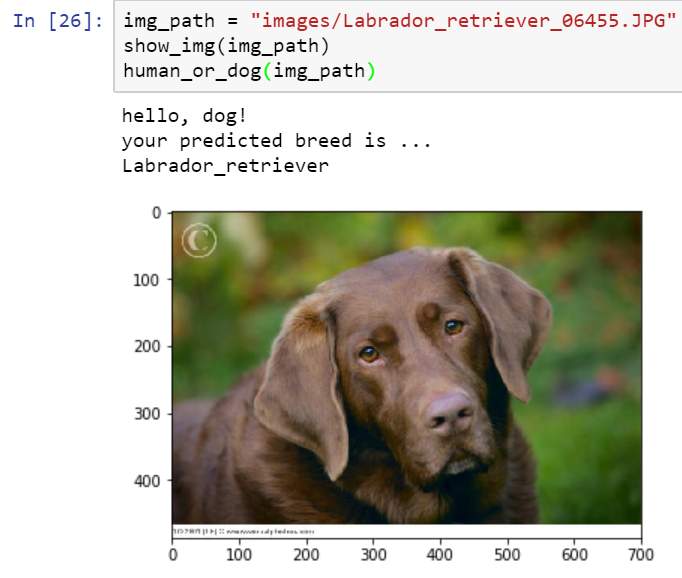
\includegraphics[width=\textwidth]{images/example0}
        \caption{Labrador Retriever}
        \label{fig:labrador_retriever}
    \end{subfigure}
    \begin{subfigure}[b]{0.3\textwidth}
        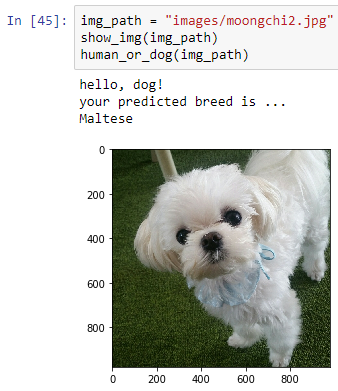
\includegraphics[width=\textwidth]{images/example1}
        \caption{Maltese}
        \label{fig:maltese}
    \end{subfigure}
    \begin{subfigure}[b]{0.3\textwidth}
        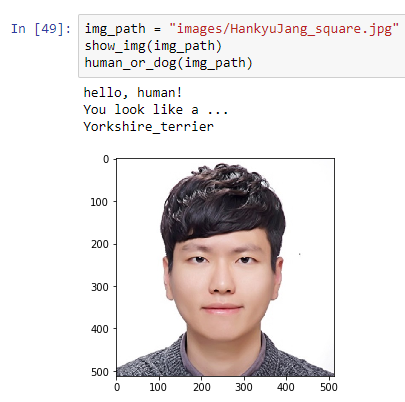
\includegraphics[width=\textwidth]{images/example2}
        \caption{Human}
        \label{fig:human}
    \end{subfigure}
    \caption{Dog Breed Prediction using CNN}\label{fig:dog_breed}
\end{figure}



\section{Revised research plan}

So far, we have attained familiarity with CNN architecture and GPU computing. We have learned how to use Big Red II for running tensorflow code and used Amazon AWS to train the models as well. For the next week, we plan to study Recurrent Neural Network and get familiar with using the network. Then, as planned before we would replicate the results of other researchers.

If we succeed, we would explore what would be the best model for the task at hand, and figure out if we want to change the architecture. We may try transfer learning; perhaps use several pre-trained models such as VGG16, VGG19, Resnet50, InceptionV3, and Xception and add one or two additional layers in the end for CNN architecture.



\bibliographystyle{unsrt}
\bibliography{report}

\end{document}